\label{pierwsze_uruchomienie}
\begin{wrapfigure}{R}{0.5\textwidth}
	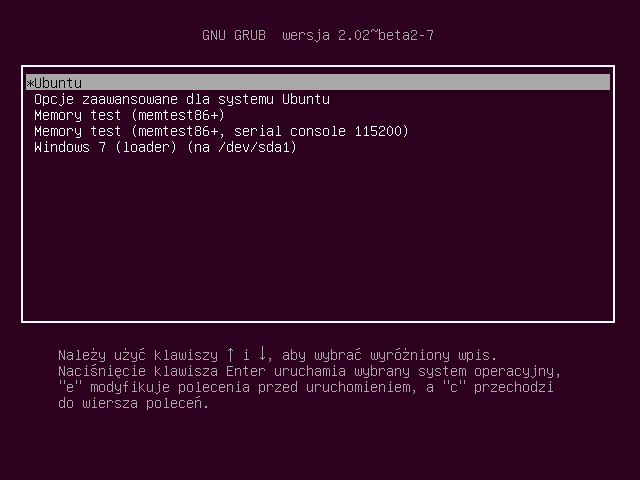
\includegraphics[width=\linewidth]{images/pierwsze_uruchomienie_grub.png}
\end{wrapfigure}

Po zainstalowaniu systemu Ubuntu twój komputer został zresetowany, zostałeś też poproszony o usunięcie nośnika instalacyjnego (pendrive, płyta DVD) z napędu. Jeżeli to wykonałeś, to przy ponownym uruchomieniu komputera powinieneś zobaczyć ekran bardzo podobny do tego. Jest to GRUB (\textcolor{ubuntu_orange}{Grand Unified Bootloader}), program rozruchowy, zajmujący się uruchomieniem systemu operacyjnego. Korzystając z GRUB-a, możesz wybrać który system operacyjny ma zostać uruchomiony. Za pomocą klawiszy kursora podświetl odpowiednią opcję i wciśnij \keys{\returnwin}.

Jeżeli Ubuntu jest jedynym systemem operacyjnym na twoim komputerze, to menu GRUB-a nie wyświetli się. Zamiast tego przez około sekundę ekran będzie ciemnofioletowy, a następnie zostanie uruchomiony system Ubuntu. Aby w takiej sytuacji wejść do menu GRUB-a, wciśnij klawisz \keys{Shift}, gdy ekran stanie się fioletowy.

\begin{itemize}
\item \textcolor{ubuntu_orange}{Opcje zaawansowane dla systemu Ubuntu}: zestaw dodatkowych programów naprawczych i diagnostycznych systemu Ubuntu (zostały one szerzej opisane w rozdziale \ref{rozwiązywanie problemów} ,,Rozwiązywanie problemów'');
\item \textcolor{ubuntu_orange}{Memorytest}: program służący do testowania pamięci operacyjnej (RAM) komputera;
\item \textcolor{ubuntu_orange}{Windows 7 Loader}: uruchamia system operacyjny Windows 7.
\end{itemize}

Ilość pozycji w menu będzie się różnić w zależności od tego, ile, i jakie systemy operacyjne masz zainstalowane na swoim komputerze.

\begin{flushright}
Wybierz \textcolor{ubuntu_orange}{Ubuntu} i wciśnij klawisz \keys{\returnwin}, aby uruchomić Ubuntu.
\end{flushright}
\clearpage
